\section{Resultados}
A continuación, mostramos los resultados obtenidos de la comparación entre los algoritmos PageRank e IN-DEG para instancias particulares. Dichos resultados son la importancia de cada página j, es decir el $x_{j}$. \\

\begin{figure}[H]
\centering     %%% not \center
\subfigure[Figure A]{\label{fig:a}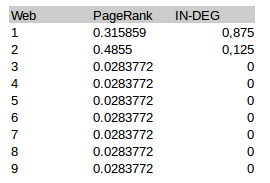
\includegraphics[width=0.4\linewidth]{imagenes/resultadosEstrella.png}}
\subfigure[Figure B]{\label{fig:b}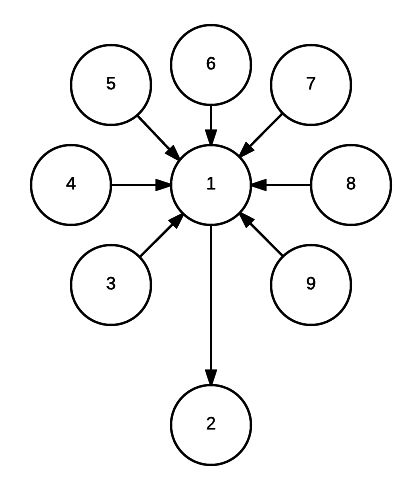
\includegraphics[width=0.3\linewidth]{imagenes/estrella.png}}
\caption{Web con estructura de estrella.}
\end{figure}

En el caso de una web con forma de estrella, cabe destacar las páginas 1 y 2. La página 1 es referenciada por todas las demás, salvo la 2 que es referenciada por la página 1. Dado que IN-DEG definie el ranking de una página j en base a la cantidad de ejes entrantes, es claro que la página uno obtenga la primer posición y la página 2 la segunda posición. Las páginas restantes tienen ranking cero por no ser referenciadas por ninguna otra.
En cambio, para PageRank se hace visible la idea de qué tan importante es el que referencia, en vez de cuantos son los que referencian. Las páginas que no son linkeadas tienen una importancia baja en comparación a las primeras dos.


\begin{figure}[H]
\centering     %%% not \center
\subfigure[Figure A]{\label{fig:a}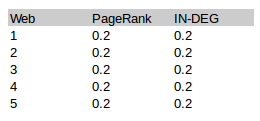
\includegraphics[width=0.4\linewidth]{imagenes/resultadosCompleto.png}}
\subfigure[Figure B]{\label{fig:b}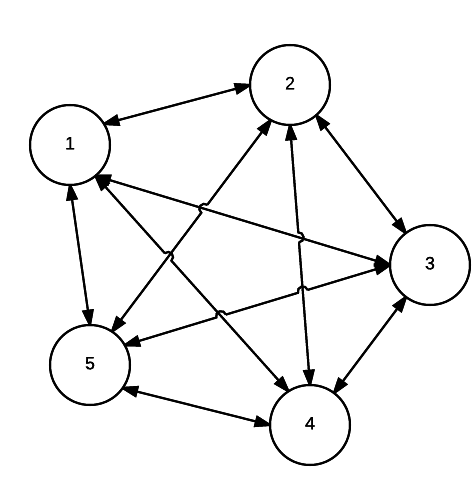
\includegraphics[width=0.3\linewidth]{imagenes/completo.png}}
\caption{Web con estructura de pentágono.}
\end{figure}

El segundo ejemplo, un grafo completo de cinco nodos, lo hicimos para encontrar los casos en que los criterios de importancia de ambos algoritmos coinciden. Era esperable que todas las páginas tengan la misma importancia en ambos dos, ya que todas las páginas web son referenciadas por páginas con la misma importancia.

\begin{figure}[H]
\centering     %%% not \center
\subfigure[Figure A]{\label{fig:a}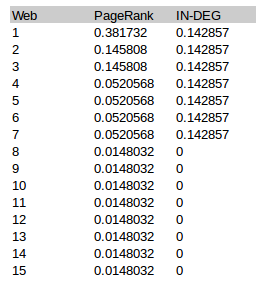
\includegraphics[width=0.3\linewidth]{imagenes/resultadosBinario.png}}
\subfigure[Figure B]{\label{fig:b}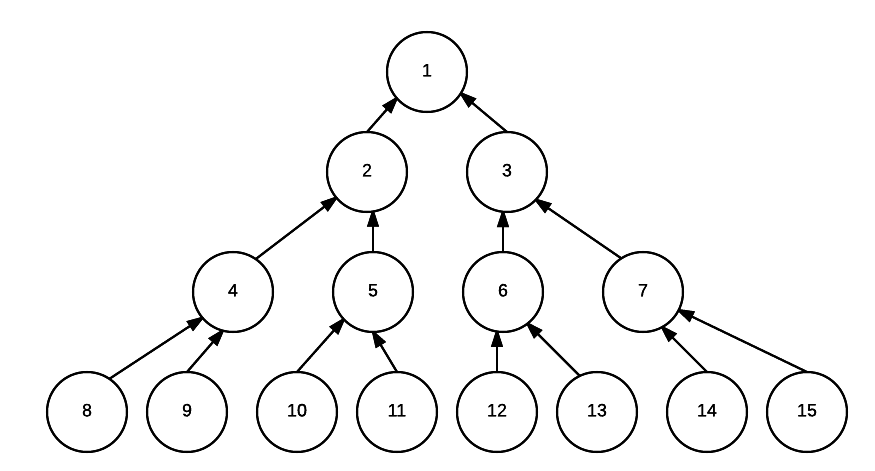
\includegraphics[width=0.5\linewidth]{imagenes/binario.png}}
\caption{my caption}
\end{figure}


\begin{figure}[H]
\centering     %%% not \center
\subfigure[Figure A]{\label{fig:a}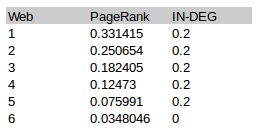
\includegraphics[width=0.4\linewidth]{imagenes/resultadosCamino.png}}
\subfigure[Figure B]{\label{fig:b}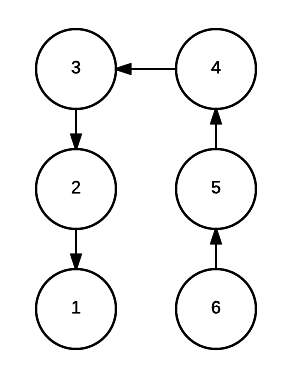
\includegraphics[width=0.2\linewidth]{imagenes/camino.png}}
\caption{my caption}
\end{figure}